
\begin{figure}[!htb]
\begin{centering}
                            % trim=left bottom right top
    % {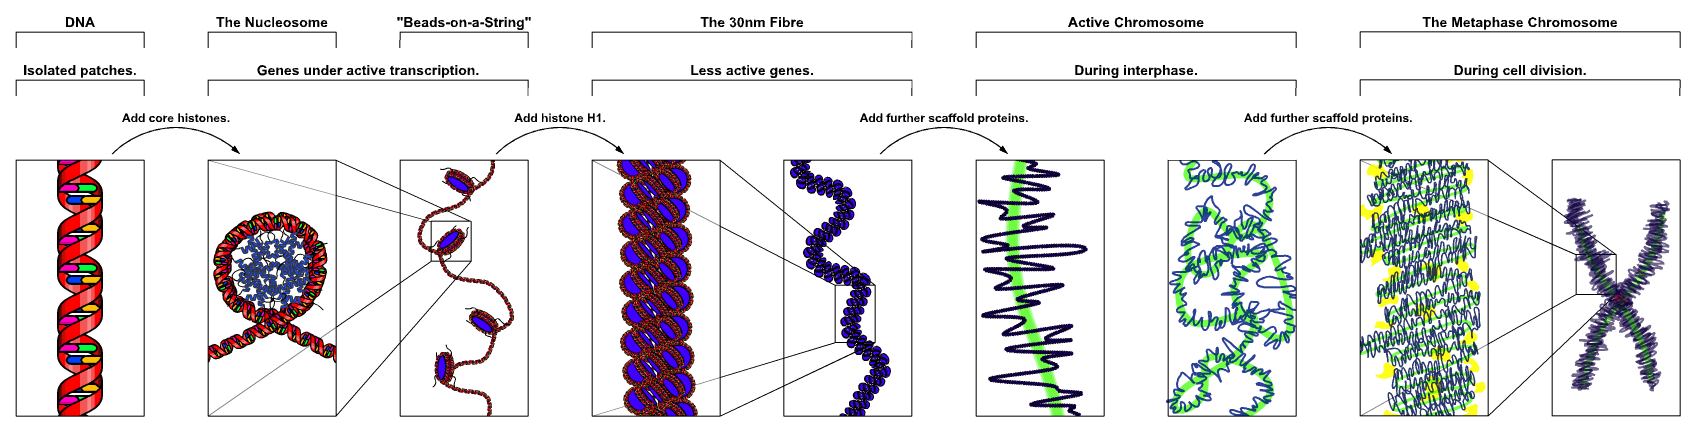
\includegraphics[scale=0.27,trim=15 0 207 155,clip]{figures/background/Chromatin_Structures}
    {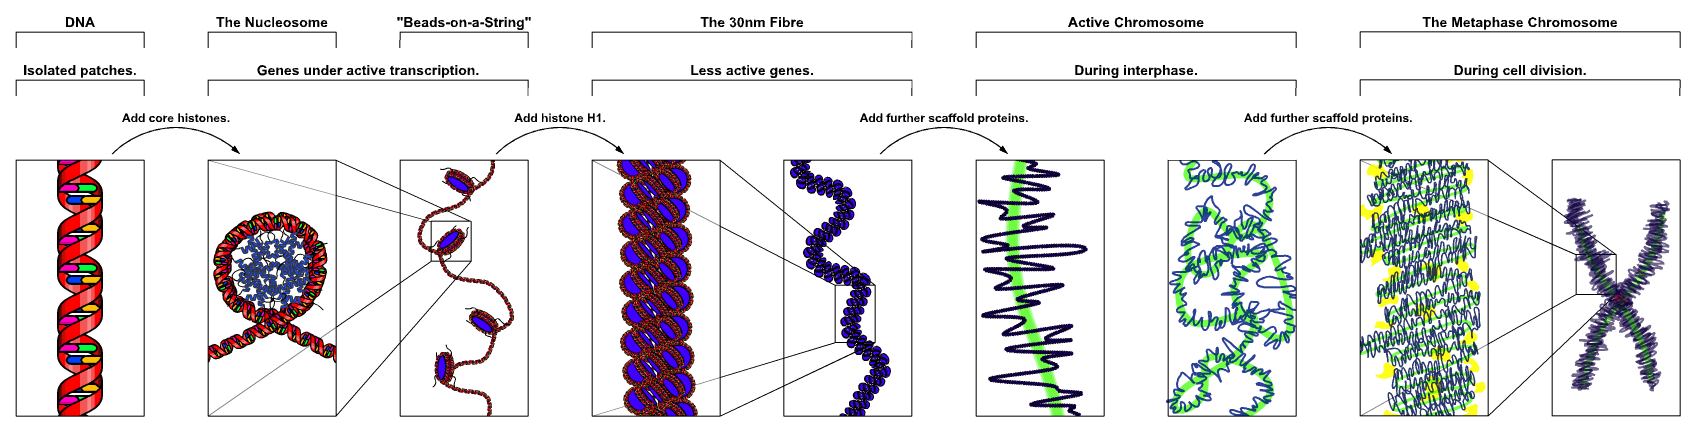
\includegraphics[scale=0.5,trim=15 0 975 155,clip]{figures/background/Chromatin_Structures}} \\
    {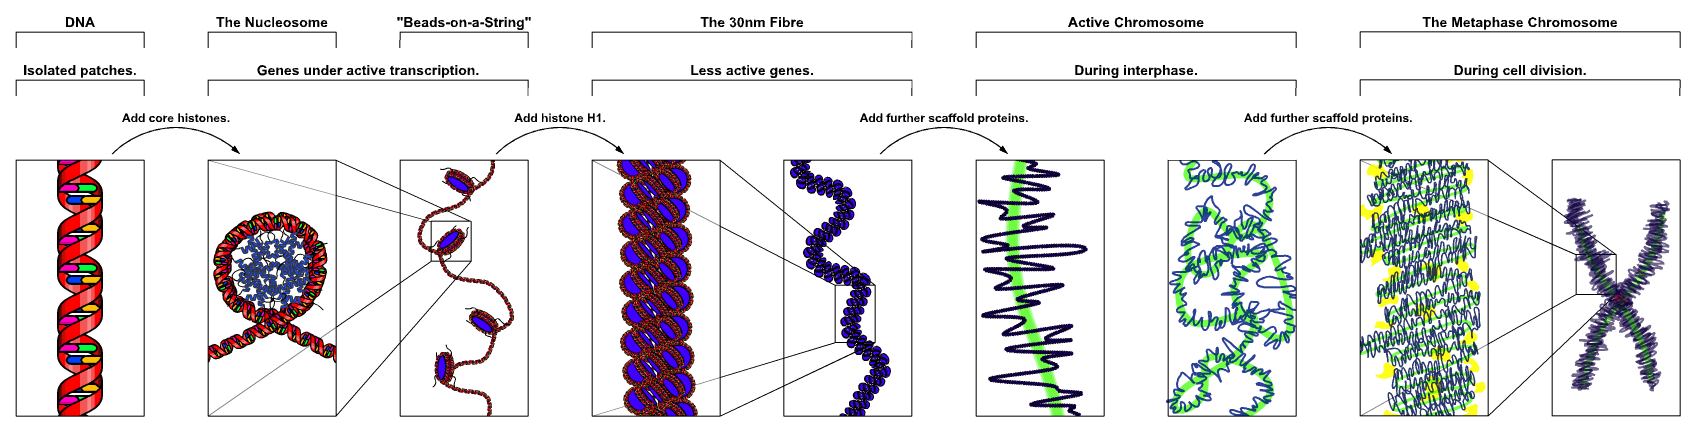
\includegraphics[scale=0.5,trim=784 0 207 155,clip]{figures/background/Chromatin_Structures}}
    \caption[Major Chromatin Structures]
    {\textbf{Major Chromatin Structures.}

    Note that not all are listed, and considerably different structures exist
    during cell division as well. These structures are representative most of the
    time. \\ \\ Image adapted from \cite{figchromatinstructures}.}
    \label{fig:comparison3C}\label{fig:chromatin}
\end{centering}
\end{figure}



